\documentclass[aspectratio=169]{beamer}
 
\usepackage[utf8]{inputenc}
\usepackage{fouriernc} % Alternative font: utopia
\usefonttheme[onlymath]{serif}

\usepackage{physics}
\usepackage{multicol}
\usepackage{bibentry}
\usepackage{url}
\bibliographystyle{abbrv}

% \usecolortheme{seahorse}
\usecolortheme{whale}
% \usecolortheme{albatross}
\setbeamerfont{footnote}{size=\fontsize{4pt}{5pt}}
\setbeamertemplate{navigation symbols}{}  % disable the navigation buttons at the bottom of the slide

\newcommand\Wider[2][3em]{%
\makebox[\linewidth][c]{%
  \begin{minipage}{\dimexpr\textwidth+#1\relax}
  \raggedright#2
  \end{minipage}%
  }%
}

% \renewcommand{\footnotesize}{\fontsize{5pt}{7pt}\selectfont}

 
\title{Computational Methods for Plasmas}
\author{Evan Bluhm}
% \institute{AA 560}
\date{May 24, 2021}
% \date[VLC 2013]{February 2021}
 
\begin{document}

%%%%%%%%%%%%%%%%%%%%%%%%%%%%%%%%%%%%%%%%%%%%%%%%%%%%%%%%%%%%%%%%%%%%%%%%%%%%%%%%
\begin{frame}
\titlepage
% Put nobibliography on the first slide so citations become available in footnotes for all following frames
\nobibliography{presentation.bib}
\end{frame}
%%%%%%%%%%%%%%%%%%%%%%%%%%%%%%%%%%%%%%%%%%%%%%%%%%%%%%%%%%%%%%%%%%%%%%%%%%%%%%%%
 
\begin{frame}
\frametitle{Magnetostatic PIC Model}

\begin{itemize}
\item 1D2V ($x$, $v_x$, $v_y$) solver. Except for the Poisson solver, the implementation mirrors the magnetostatic ES1 described in Birdsall.
\item Uses 0th and 1st order weighting functions.
\item Poisson's equation solved using implicit finite difference method, with optional FFT method implemented.
\item Same normalization as ES1: time, charge, mass, and magnetic field normalized by input parameters $\omega_p$, $q/m$, $\epsilon_0$, and $B_0$. Spatial normalization left to the initial conditions.
\end{itemize}

\end{frame}
%%%%%%%%%%%%%%%%%%%%%%%%%%%%%%%%%%%%%%%%%%%%%%%%%%%%%%%%%%%%%%%%%%%%%%%%%%%%%%%%
\begin{frame}
\frametitle{PIC: Code Structure}
\Wider{
\begin{figure}[h]
\centering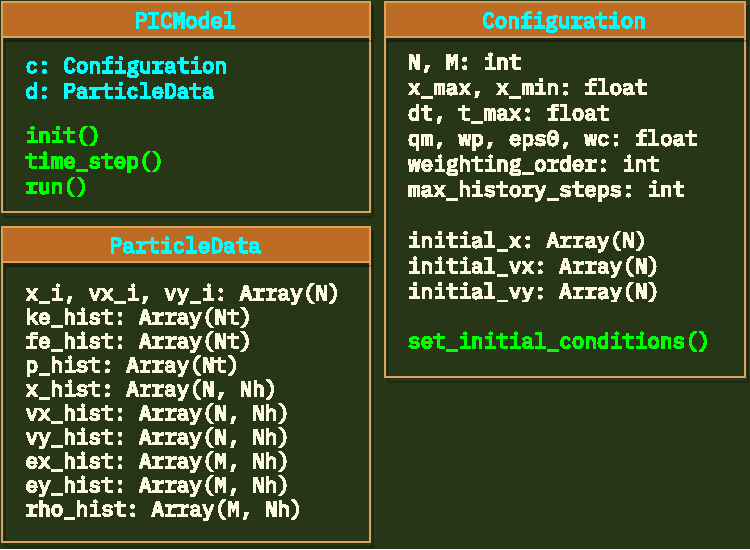
\includegraphics[width=0.7\paperwidth]{presentation/classdiagram-pic.pdf}
% \footnote{\bibentry{wiki:zeeman-splitting-breit-rabi}}
\end{figure}
}
\end{frame}

% % %%%%%%%%%%%%%%%%%%%%%%%%%%%%%%%%%%%%%%%%%%%%%%%%%%%%%%%%%%%%%%%%%%%%%%%%%%%%%%%%

\begin{frame}
\frametitle{PIC: Demos}

\begin{itemize}
\item Langmuir oscillations
\begin{itemize}
    \item Simplest 1D oscillations. ``Kicking the tires.''
\end{itemize}
\item Two-stream instability
\begin{itemize}
    \item Important result to reproduce for electrostatic codes.
    \item Also lends itself to flashy animations.
\end{itemize}
\item Dory-Guest-Harris instability
\begin{itemize}
    \item Test of the magnetostatic capabilities.
    \item Grid spacing convergence test.
\end{itemize}
\end{itemize}

\end{frame}

% % %%%%%%%%%%%%%%%%%%%%%%%%%%%%%%%%%%%%%%%%%%%%%%%%%%%%%%%%%%%%%%%%%%%%%%%%%%%%%%%%
 
\begin{frame}
\frametitle{MHD Finite Difference Solver}

\begin{itemize}
\item Full 3D spatial grid
\item Stability \& accuracy checks: CFL condition, $\div \vec B$, positive-definite $\rho$
\item Constant artificial diffusion $\sigma \nabla ^2 Q$
\end{itemize}

\end{frame}

% % %%%%%%%%%%%%%%%%%%%%%%%%%%%%%%%%%%%%%%%%%%%%%%%%%%%%%%%%%%%%%%%%%%%%%%%%%%%%%%%%

\begin{frame}
\frametitle{MHD: Code Structure}
\Wider{
\begin{figure}[h]
\centering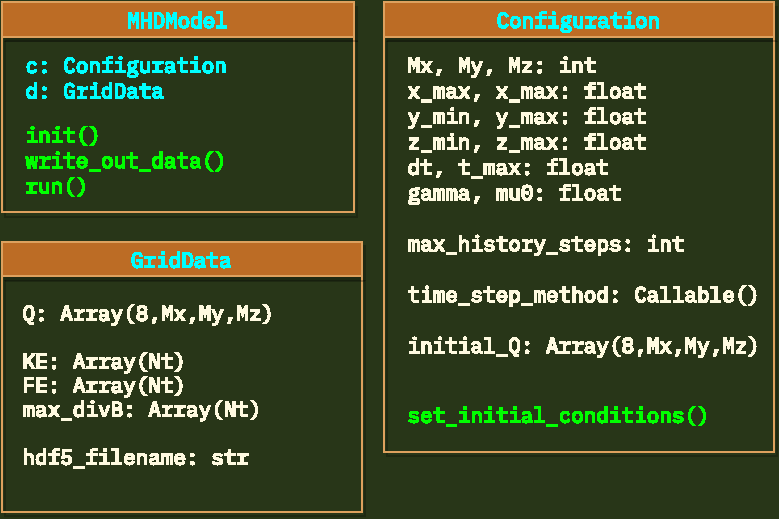
\includegraphics[width=0.7\paperwidth]{presentation/classdiagram-mhd.pdf}
% \footnote{\bibentry{wiki:zeeman-splitting-breit-rabi}}
\end{figure}
}
\end{frame}

% % %%%%%%%%%%%%%%%%%%%%%%%%%%%%%%%%%%%%%%%%%%%%%%%%%%%%%%%%%%%%%%%%%%%%%%%%%%%%%%%%
 
\begin{frame}
\frametitle{MHD: Demos}

\begin{itemize}
\item Brio-Wu Shock Tube
\begin{itemize}
    \item MHD equivalent of Sod's shock tube problem. Generates a variety of waves, and tests how the solver handles shocks.
    \item Brio, M. \& C.C. Wu, ``An Upwind Differencing Scheme for the Equations of Ideal Magnetohydrodynamics'', Journal of Computational Physics, 75, 400-422 (1988).
\end{itemize}
\item Screw Pinch Equilibrium
\end{itemize}

\end{frame}

% % %%%%%%%%%%%%%%%%%%%%%%%%%%%%%%%%%%%%%%%%%%%%%%%%%%%%%%%%%%%%%%%%%%%%%%%%%%%%%%%%
 
\begin{frame}
\frametitle{Questions?}

Brought to you by:

\centering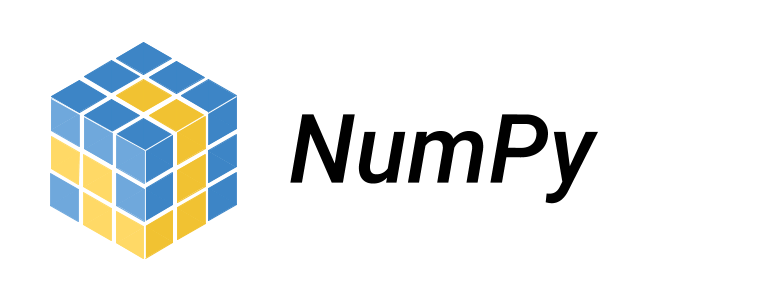
\includegraphics[width=0.3\paperwidth]{presentation/numpy.png} 
\includegraphics[width=0.3\paperwidth]{presentation/numba.png}

\includegraphics[width=0.3\paperwidth]{presentation/tutorial_matplotlib.png}

\end{frame}
% %%%%%%%%%%%%%%%%%%%%%%%%%%%%%%%%%%%%%%%%%%%%%%%%%%%%%%%%%%%%%%%%%%%%%%%%%%%%%%%%

\end{document}